%%%%%%%%%%%%%%%%%%%%%%%%%%%%%%%%%%%%%%%%%
% Short Sectioned Assignment
% LaTeX Template
% Version 1.0 (5/5/12)
%
% This template has been downloaded from:
% http://www.LaTeXTemplates.com
%
% Original author:
% Frits Wenneker (http://www.howtotex.com)
%
% License:
% CC BY-NC-SA 3.0 (http://creativecommons.org/licenses/by-nc-sa/3.0/)
%
%%%%%%%%%%%%%%%%%%%%%%%%%%%%%%%%%%%%%%%%%
\documentclass[paper=a4, fontsize=11pt]{scrartcl} % A4 paper and 11pt font size
\usepackage[T1]{fontenc}
\usepackage{fourier}
\usepackage[english]{babel}
\usepackage{amsmath,amsfonts,amsthm}

\usepackage{lipsum}

\usepackage{sectsty}
\allsectionsfont{\centering \normalfont\scshape}

\usepackage{fancyhdr}
\pagestyle{fancyplain}
\fancyhead{}
\fancyfoot[L]{} % Empty left footer
\fancyfoot[C]{} % Empty center footer
\fancyfoot[R]{\thepage} % Page numbering for right footer
\renewcommand{\headrulewidth}{0pt} % Remove header underlines
\renewcommand{\footrulewidth}{0pt} % Remove footer underlines
\setlength{\headheight}{13.6pt} % Customize the height of the header

\numberwithin{equation}{section}
\numberwithin{figure}{section}
\numberwithin{table}{section}

\setlength\parindent{0pt}

\usepackage{graphicx}
\graphicspath{ {./images/} }

\usepackage{listings}
\usepackage{color}

\definecolor{dkgreen}{rgb}{0,0.6,0}
\definecolor{gray}{rgb}{0.5,0.5,0.5}
\definecolor{mauve}{rgb}{0.58,0,0.82}

\lstset{frame=tb,
  language=Java,
  aboveskip=5mm,
  belowskip=3mm,
  showstringspaces=false,
  columns=flexible,
  basicstyle={\small\ttfamily},
  numbers=none,
  numberstyle=\tiny\color{gray},
  keywordstyle=\color{blue},
  commentstyle=\color{dkgreen},
  stringstyle=\color{mauve},
  breaklines=true,
  breakatwhitespace=true,
  tabsize=3
}

%----------------------------------------------------------------------------------------
%	TITLE SECTION
%----------------------------------------------------------------------------------------

\newcommand{\horrule}[1]{\rule{\linewidth}{#1}} % Create horizontal rule command with 1 argument of height

\title{	
\normalfont \normalsize 
\horrule{0.5pt} \\[0.4cm] % Thin top horizontal rule
\huge Week 03 \\ % The assignment title
\horrule{2pt} \\[0.5cm] % Thick bottom horizontal rule
}

\author{Seth Childers} % Your name

\date{} % Today's date or a custom date

\begin{document}

\maketitle % Print the title

%----------------------------------------------------------------------------------------
%	PROBLEM 1
%----------------------------------------------------------------------------------------

\section{3-1 Exercise 01}

\textbf{Problem:}

\textit{a.} Give an example of an algorithm that should not be considered an application of the brute-force approach.

\textit{b.} Give an example of a problem that cannot be solved by a brute-force algorithm.

\bigskip
\textbf{Code written in Python}
\begin{lstlisting}
#######################################################################
# Exercises 3.1 - #01
# a. Give an example of an algorithm that should not be 
# considered an application of the brute-force approach.
#
# A binary search is an example of an algorithm that should
# not be considered for a brute-force approach. This is
# because the binary search is used to find a single item
# that matches what you are looking for, where going through
# each element would be inefficient and unnecessary. 
#
# b. Give an example of a problem that cannot be solved
# by a brute-force algorithm.
#
# A problem that cannot be solved by a brute-force algorithm
# is one that solves for the next best set of moves for a 
# particular card or board game. This is not feasible because
# certain games have so many possible plays each move, and calculating
# the probability of each opponent's most likely moves means that
# the possibilities for a set of moves is incredibly exponential.
# This is possible for simpler games, but machine learning is necessary
# for the more complex games in order to cut down on computations.
#######################################################################
\end{lstlisting}
\pagebreak

%----------------------------------------------------------------------------------------
%	PROBLEM 2
%----------------------------------------------------------------------------------------

\section{3-1 Exercise 08}

\textbf{Problem:} Sort the list E, X, A, M, P, L, E in alphabetical order by selection sort

\bigskip
\textbf{Code written in Python}
\begin{lstlisting}
############################################################################
# Exercises 3.1 - #08
# 
# Sort the list E, X, A, M, P, L, E in alphabetical order by selection sort
############################################################################
import sys

# Got help from https://www.geeksforgeeks.org/selection-sort/
def selectionSort(unsorted):
    for i in range(len(unsorted)):
        nextIndex = i
        for j in range(i+1, len(unsorted)):
            if unsorted[nextIndex] > unsorted[j]:
                nextIndex = j

        unsorted[i], unsorted[nextIndex] = unsorted[nextIndex], unsorted[i]

    print("Sorted array")
    for i in range(len(unsorted)):
        print("{}".format(unsorted[i] ))

unsorted = ['E', 'X', 'A', 'M', 'P', 'L', 'E']
selectionSort(unsorted)
\end{lstlisting}

\textbf{Results}
\begin{lstlisting}
Sorted array
A
E
E
L
M
P
X
\end{lstlisting}

\pagebreak

%----------------------------------------------------------------------------------------
%	PROBLEM 3
%----------------------------------------------------------------------------------------

\section{3.4 Exercise 06}

\textbf{Problem:} Odd pie fight - There are n>= 3 people positioned on a field (Euclidean plane) so that each has a unique nearest neighbor. Each person has a cream pie. At a signal, everbody hurls his or her pie at the nearest neighbor. Assuming that n is odd and that nobody can miss his or her target, true or false: There always remains at least one person not hit by a pie.

\bigskip
\textbf{Code written in Python}
\begin{lstlisting}
############################################################################
# Exercises 3.4 - #06
# 
# Odd pie fight - There are n>= 3 people positioned on a field (Euclidean plane)
# so that each has a unique nearest neighbor. Each person has a cream pie.
# At a signal, everbody hurls his or her pie at the nearest neighbor. Assuming
# that n is odd and that nobody can miss his or her target, true or false:
# There always remains at least one person not hit by a pie.
#
# True, no matter what there will always be at least one person not hit by a
# pie because the two people that have the smallest distance between them will
# hit each other, instead of hitting other people, which will throw off the
# possibility to hit everyone.
############################################################################

\end{lstlisting}

\pagebreak

%----------------------------------------------------------------------------------------
%	PROBLEM 4
%----------------------------------------------------------------------------------------

\section{3-5 Exercise 04}

\textbf{Problem:} 

\bigskip
\textbf{Code written in Python}
\begin{lstlisting}
########################################################################
# Exercises 3.5 - #04
#
# Traverse the graph of Problem 1 by breadth-first search and construct
# the corresponding breadth-first search tree. Start the traversal at 
# vertex 'a' and resolve ties by the vertex alphabetical order.
#
# Problem 1 graph:
# f --- b     c --- g
#  \   / \   /     /
#    d --- a ---- e
########################################################################
import matplotlib as plt
import networkx as nx

def main():
    # make the graph
    graph = createGraph()
    # print the graph info
    print(nx.info(graph))
    # draw and show the graph
    drawGraph(graph)
    # print out the breadth first search info
    print(list(breadthFirst(graph)))

def breadthFirst(graph):
    return nx.bfs_edges(graph, 'a')

def drawGraph(graph):
    # draw the graph
    nx.draw(graph, with_labels=True)
    # show the graph
    plt.pyplot.savefig('3-5_graph.png')

def createGraph():
    G = nx.Graph()
    G.add_nodes_from(['a', 'b', 'c', 'd', 'e', 'f', 'g'])
    G.add_edges_from([('a', 'c'), ('a', 'b'), ('a', 'e'), ('a', 'd')])
    G.add_edges_from([('d', 'f'), ('d', 'b'), ('f', 'b')])
    G.add_edges_from([('c', 'g'), ('a', 'e'), ('e', 'g')])

    return G

if __name__ == "__main__":
    main()
\end{lstlisting}

\bigskip
\textbf{Results}
\begin{lstlisting}
Type: Graph
Number of nodes: 7
Number of edges: 9
Average degree:   2.5714
[('a', 'c'), ('a', 'b'), ('a', 'e'), ('a', 'd'), ('c', 'g'), ('b', 'f')]
\end{lstlisting}

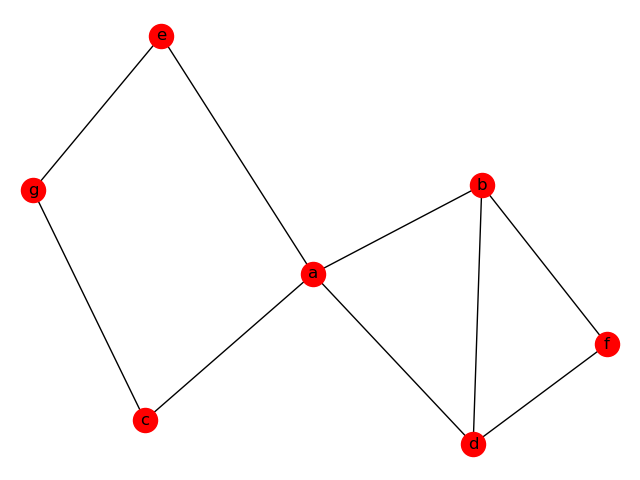
\includegraphics[width=15cm, height=10cm]{./3-5Exercise04}
\pagebreak

%----------------------------------------------------------------------------------------
%	PROBLEM 5
%----------------------------------------------------------------------------------------

\section{3-5 Exercise 08}

\textbf{Problem:} A graph is said to be bipartite if all its vertices can be partitioned into two disjoint subsets X and Y so that every edge connects a vertex in X with a vertex in Y. (One can also say that a graph is bipartite if its vertices can be colored in two colors so that every edge has its vertices colored in different colors; such graphs are also called 2-colorable.)

\textit{a.} Design a DFS-based algorithm for checking whether a graph is bipartite.

\textit{b.} Design a BFS-based algorithm for checking whether a graph is bipartite.

\bigskip
\textbf{Code written in Python}
\begin{lstlisting}
########################################################################
# Exercises 3.5 - #08
#
# A graph is said to be bipartite if all its vertices can be partitioned 
# into two disjoint subsets X and Y so that every edge connects a vertex
# in X with a vertex in Y. (One can also say that a graph is bipartite if 
# its vertices can be colored in two colors so that every edge has its 
# vertices colored in different colors; such graphs are also called
# 2-colorable.)
# For example, graph (i) is bipartite while graph (ii) is not.
#
#        (i)                              (ii)
#  x1 --- y1 --- x3                     a --- b
#  |      |      |                      |  /  |
#  y2 --- x2 --- y3                     c --- d
#
# a. Design a DFS-based algorithm for checking whether a graph is bipartite.
#   - While there is a next element to search AND the next element is not
#     the same color as the current element AND you haven't found what you're
#     looking for, go to the next element.
# b. Design a BFS-based algorithm for checking whether a graph is bipartite.
#   - While there are child nodes to search AND all child nodes are not the
#     same color as the current node AND you haven't found what you're looking
#     for, go to the next element.
########################################################################
\end{lstlisting}
\pagebreak
%----------------------------------------------------------------------------------------
%	PROBLEM 6
%----------------------------------------------------------------------------------------

\section{Barney 2.6}

\textbf{Problem:} 

\bigskip
\textbf{Code written in JavaScript}
\begin{lstlisting}
/**
 * Exercise 2.6 - Find the Door
 * 
 * You are facing a wall that stretches innitely in both directions.
 * There is a door in the wall, but you know neither how far away nor in
 * which direction. You can see the door only when you are right next to it.
 * Design and write code for an algorithm that enables you to reach the door 
 * by walking at most O(n) steps where n is the (unknown to you) number of 
 * steps between your initial position and the door. (Hint: walk alternately 
 * right and left going each time exponentially farther from your initial 
 * position.)
 * 
 * @param {number} stepsToTake 
 * @param {number} doorLocation 
 */
function findDoor(stepsToTake, doorLocation) {
    let found = false;
    let stepsTaken = 0;
    let currentLocation = 0;
    while (!found) {
        stepsToTake++;
        currentLocation += stepsToTake;
        stepsTaken += stepsToTake;
        if (doorLocation < stepsToTake && doorLocation > 0) found = true;
        currentLocation -= stepsToTake * 2;
        stepsTaken += stepsToTake * 2;
        if (doorLocation > stepsToTake && doorLocation < 0) found = true;
        currentLocation += stepsToTake;
        stepsTaken += stepsToTake;
    }
    return stepsTaken;
}

const doorLocation = Math.floor(Math.random() * 100);
console.log(`Number of back and forths to find the door at spot ${doorLocation}: ${findDoor(1, doorLocation)}`);

\end{lstlisting}

\bigskip
\textbf{Results}
\begin{lstlisting}
Number of back and forths to find the door at spot 13: 416
\end{lstlisting}

\pagebreak
%----------------------------------------------------------------------------------------

\end{document}